% report.tex - HPC 714 Report
% Uncomment the below line for the double spaced, review copy
% \documentclass[draftclsnofoot,onecolumn,conference,11pt]{IEEEtran}
% Uncomment the below line for the two column, final copy
\documentclass[conference,twocolumn,11pt]{IEEEtran}

% Load packages for the report
\usepackage{cite}
\usepackage{array}
\usepackage[caption=false,font=normalsize,labelfont=sf,textfont=sf]{subfig}
\usepackage{url}

% Graphics and figures configuration
\usepackage[pdftex]{graphicx}
% declare the path(s) where your graphic files are
\graphicspath{{./figures/}}
% and their extensions so you won't have to specify these with
% every instance of \includegraphics
\DeclareGraphicsExtensions{.pdf,.jpeg,.png}

% Math package configuration
\usepackage{amsmath}
\interdisplaylinepenalty=2500

% correct bad hyphenation here
\hyphenation{op-tical net-works semi-conduc-tor}


\begin{document}

% report title
\title{Actors for Distributed Dataflow}


% author names and affiliations
\author{
    \IEEEauthorblockN{Benjamin Bengfort}
    \IEEEauthorblockA{
    \textit{University of Maryland}\\
    Department of Computer Science\\
    Email: bengfort@cs.umd.edu\\
    }

    \and
    \IEEEauthorblockN{Allen Leis}
    \IEEEauthorblockA{\textit{University of Maryland}\\
    Department of Computer Science\\
    Email: aleis@umd.edu\\
    }

    \and
    \IEEEauthorblockN{Konstantinos Xirogiannopoulos}
    \IEEEauthorblockA{\textit{University of Maryland}\\
    Department of Computer Science\\
    Email: kostasx@cs.umd.edu\\
}}

% make the title area
\maketitle

% report abstract
\begin{abstract}
Recently, the Actor model of concurrency in distributed systems has regained popularity as cluster computing frameworks for large scale analytics have become mainstream. In particular, the use of virtual actors provides automatic scaling and load balancing through virtual actor properties of perpetual existence, automatic instantiation, and locale transparency. This programming model is ideal for data processing of streams of unbounded data sets, in a computing architecture of live, online processing of data. In this paper, we present the communication patterns of three such data processing applications as casts of Actors. We then model the communication behavior on a cluster using a simulation and show that the actor model effectively describes how a cluster should behave in response to variable volumes of data. We propose that this simulation motivates the future work of generalizing virtual actor spaces for distributed computation.
\end{abstract}

\section{Introduction}

Sensors, web logs, and other timely data sources are increasingly being used for  real-time or on-demand applications that utilize machine learning models to quickly make predictions and adapt to changes reflected by the input data. Timely sources present a challenge as they are streams of unbounded, occasionally unordered data sets that must be computed upon in an online fashion rather than in batch. When these data sources are also variable (e.g. the volume of traffic can spike) then the underlying computing framework must be able to scale and balance the load or risk falling so far behind that the computation becomes meaningless.

Because of the widespread adoption of distributed computing frameworks like MapReduce \cite{dean_mapreduce:_2008} and Spark \cite{zaharia_resilient_2012}, distributed computing in a cluster of (often virtualized) economic servers has become the default, general method of high performance data processing. These frameworks primarily abstract the details of parallelism and distributing computation away from the developer, and have allowed a wider community of programmers and scientists to take advantage of parallel algorithms and libraries. Machine learning in particular has come of age in this computing environment, and as a result there exist many high level libraries for fitting a wide array of models in parallel.

As a result, tools for dealing with \textit{streaming data} (unbounded, unordered, variable data sources) have mostly been contextualized similarly to parallel machine learning algorithms -- via descriptions of how data flows through the application. Tools like Spark Streaming \cite{zaharia_discretized_2012}, Storm \cite{toshniwal_storm_2014}, and Google DataFlow \cite{akidau_dataflow_2015} implement a \textit{data flow} programming model, where analysis is described as a directed graph whose nodes represent a single computation, and whose edges represent the transmission of input and output values. Describing computation this way is simple, adaptable, and when mapped to a distributed topology, scalable. However, this model does not allow nodes to communicate, nor provide any flexibility in the computational topology for error handling, transactional guarantees, consistency, or persistence.

In response to the inflexibility of the data flow model, the \textit{actor model} \cite{hewitt_viewing_1977, agha_actors:_1985} has been re-emerging as an abstraction that allows for flexible communication between distributed processes while still at a high enough level to abstract the details of communication in the cluster away from the programmer. Ironically, it is this model that underpins the more general data flow models \cite{gonzalez_asynchronous_2015}, perhaps due to the fact that these applications are implemented in the Scala programming language, which by default uses actors for concurrency \cite{haller_scala_2009,karmani_actor_2009}. Actors in this context are high level primitives that do not share state, making them ideal candidates for under-the-hood parallelism. However, a simple data structure alone is not enough for a distributed computing, there must also be an execution and job management context. Orleans \cite{bernstein_orleans:_????} presents the idea of a ``virtual actor space'', analogous to virtual memory, such that actor instances (e.g. instances of a program) exist forever, are transparent to their locale, and are automatically instantiated and deactivated. Virtual actors therefore provide for automatic scaling and load balancing in the cluster, and are a novel replacement for the data flow model in the context of online, streaming computation.

In this paper we investigate the potential of virtual actors for distributed computing on streaming data by simulating a computing cluster which implements a \textit{generalized virtual actor space}. A generalized virtual actor space replaces the programing model of virtual actors with a daemon service that runs in the background of all nodes in the cluster; allocating resources to a variety of actor programs in an on-demand fashion such that the resources can scale as variable streams of data spike, while balancing load across many ``always on'' computations that must share resources. We have simulated this framework by analyzing the communications patterns of three real-time applications: a traditional data flow, an online recommendation application, and a solar weather forecasting application. We then present an analysis of how the virtual actor model behaved in simulation on the cluster and show that this model is a suitable substitute for the data flow model.

The rest of this paper is organized as follows. In the first section we will present the details of our distributed computing model using actors, and describe the generalized virtual actor space in detail. Following this, we will describe the applications we analyzed, and how we built a communications model from each type of application. Finally, we will describe our simulation methodology, present our results, and conclude with a discussion and future work.

\section{Distributed Computing Framework}

This section describes a distributed computing framework that utilizes \textit{virtual actors} and its implementation for handling always-on computations that deal with streaming data. This framework sets the stage for the analysis of applications and their communications patterns and informs the construction of the simulation.

\subsection{Actors for Concurrency}

Actors are a model for reasoning about concurrent computation which is inspired by the \textit{communication mechanisms} of a society of experts that engage in effective problem solving \cite{hewitt_viewing_1977}.  Like other distributed models, actors are event oriented where events are received messages from other actors, and therefore parallelism is demonstrated through the partial ordering of events. At a higher level, actors can be seen as data or task parallel pieces of a larger overall computation which maintain their state (e.g. each actor is a SPMD program).

% TODO: Kostas can you take this part?

Actors embody the three fundamental properties of computation: (1) storage, (2) processing or state change, (3) communication.

Actor model MIT dissertation \cite{hewitt_viewing_1977, agha_actors:_1985}


\subsection{Generalized Virtual Actor Space}

% TODO: Kostas, can you take a swing at this while I'm dealing with kids?

Orleans \cite{bernstein_orleans:_????}

\begin{figure}[!h]
    \centering
    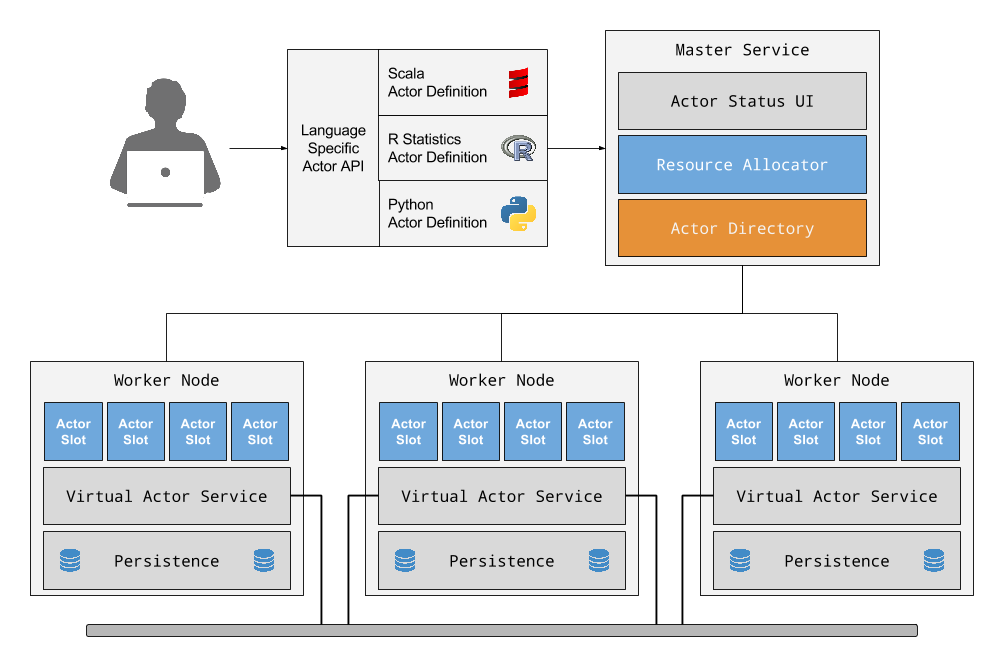
\includegraphics[width=0.45\textwidth]{architecture}
    \caption{The architecture for a generalized virtual actor framework.}
    \label{fig:architecture}
\end{figure}

\section{Applications Analysis}

% This paragraph is pretty fundamental
In order to show that a generalized virtual actor framework is a distributed programming abstraction well suited to handling streaming data for online applications we must show two things: (1) that the model is a high level abstraction, friendly to programmers but providing powerful concurrent guarantees and (2) that the model can be applied to real world problems in an efficient and robust manner. We hope to have shown the former in the last section where we described how programs are built using the actor framework. In this section, we explore the latter by analyzing three streaming applications and how they would be adapted to the actor model.

\subsection{Email Analysis Data Flow}

Heron, \cite{kulkarni_twitter_2015}
Storm, \cite{toshniwal_storm_2014}

DStreams, \cite{zaharia_discretized_2012}

\begin{figure}[!h]
    \centering
    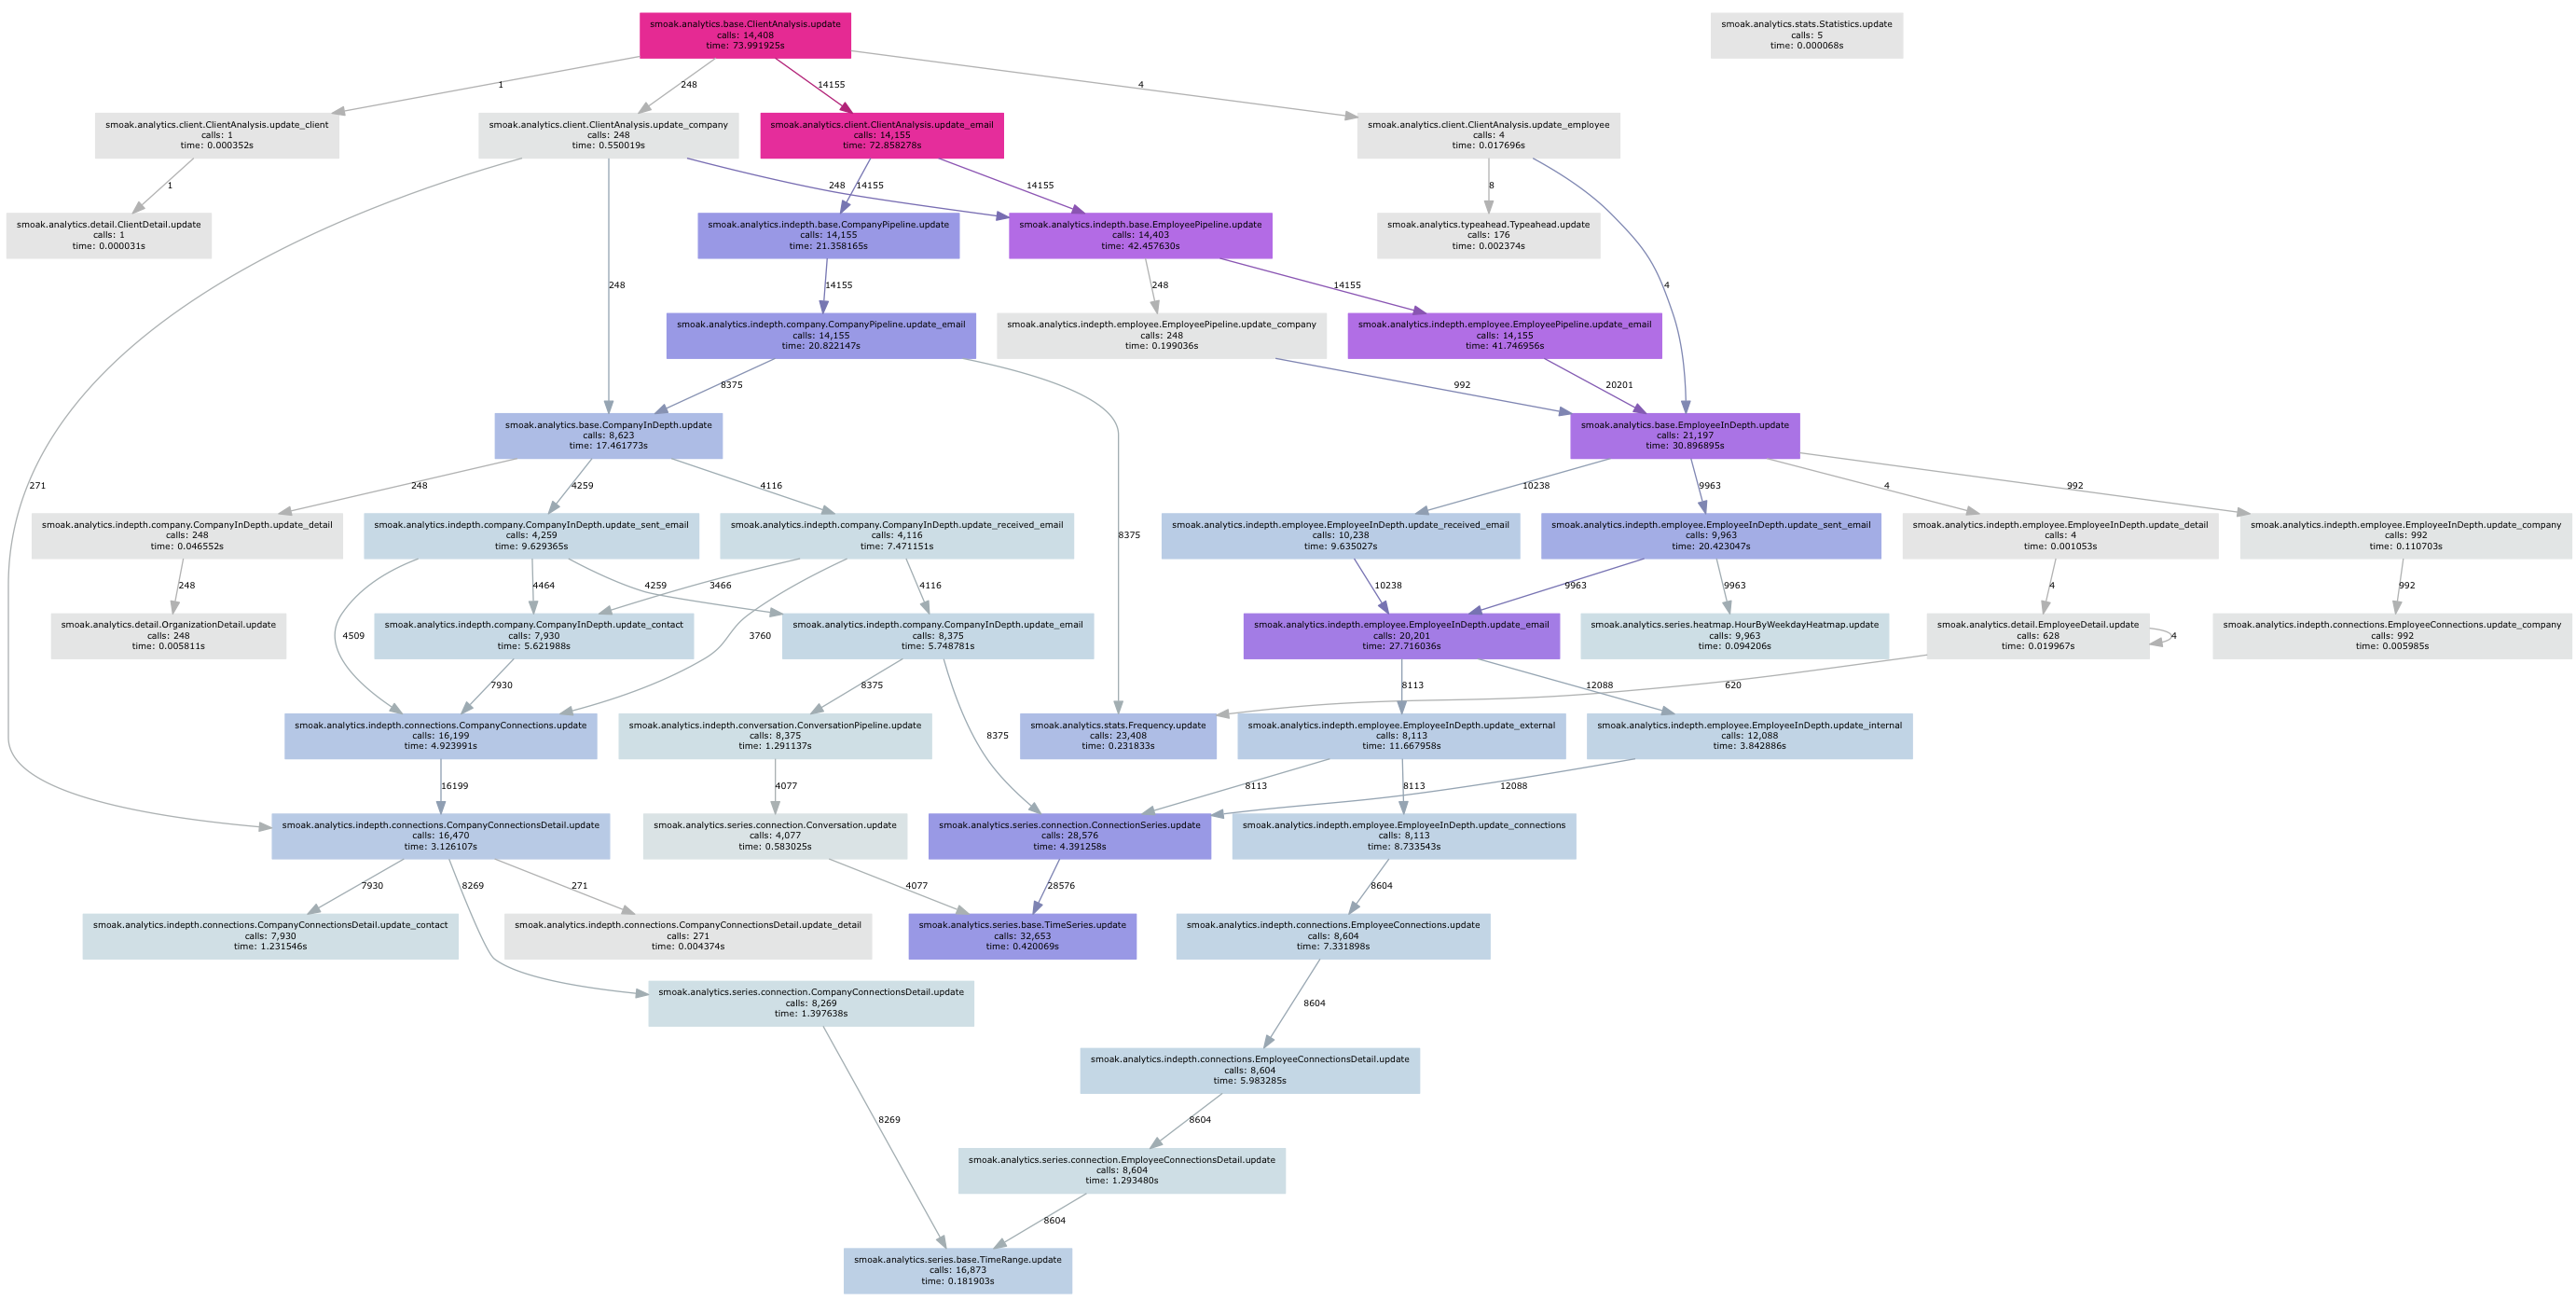
\includegraphics[width=0.45\textwidth]{dataflow_cast}
    \caption{The actor cast for a typical dataflow program.}
    \label{fig:dataflow_cast}
\end{figure}

\subsection{Online Recommendations}

Parallel sparse matrix factorization \cite{gupta_highly_1997}
Coordinate Descent factorization \cite{yu_scalable_2012}
Distributed SGD \cite{gemulla_large-scale_2011}

\begin{figure}[!h]
    \centering
    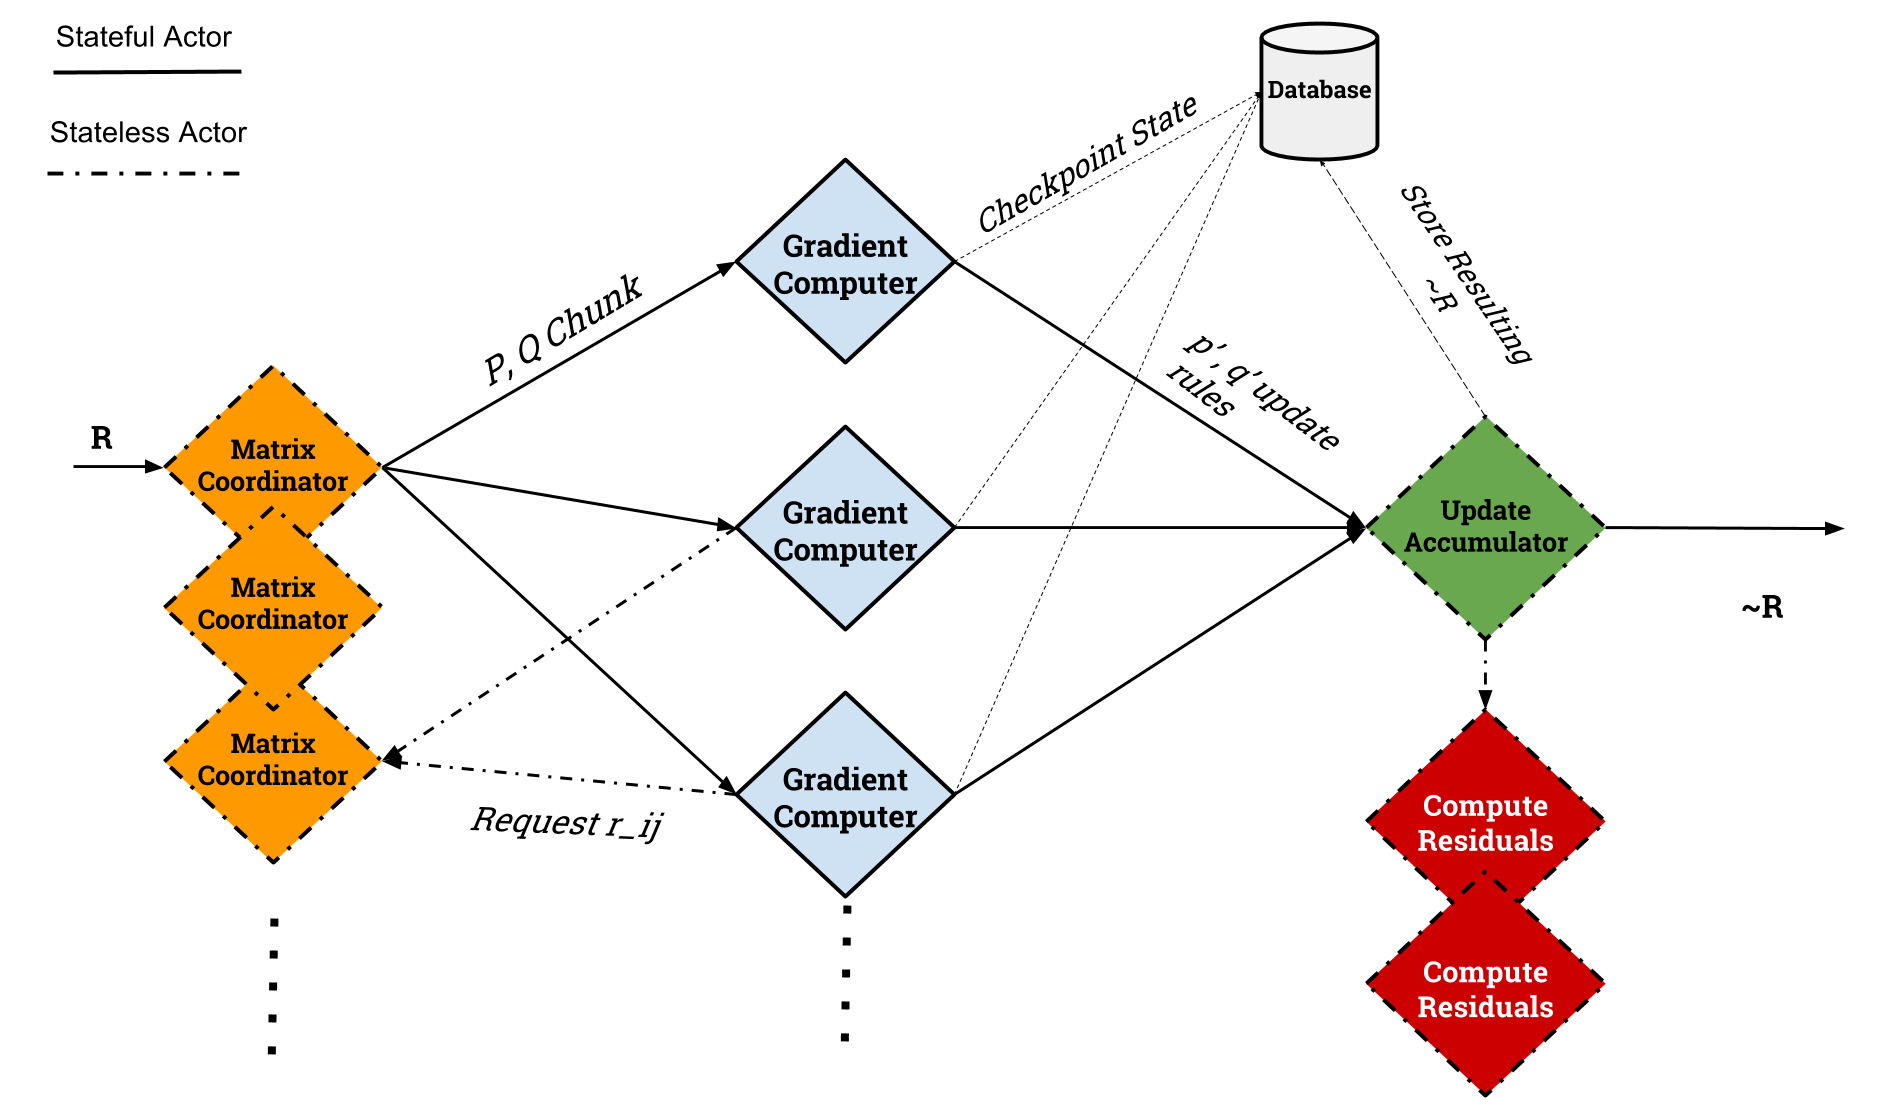
\includegraphics[width=0.45\textwidth]{nnmf_cast}
    \caption{The actor cast for implementing online recommendations with matrix factorization.}
    \label{fig:nnmf_cast}
\end{figure}

\subsection{USGS Magnetometer Prediction}

Bayesian anomaly detection in sensor networks \cite{hill_real-time_2007}
Downpour SGD \cite{dean_large_2012}
A Bayesian approach to solar flare prediction \cite{wheatland_bayesian_2004}
Solar Flare prediction using machine learning \cite{qahwaji_automatic_2007}
Solar Flare Prediction using short term sequential approach \cite{yu_short-term_2009}
Solar Flare Prediction using multiresolution predictors \cite{yu_short-term_2010}

\begin{figure}[!h]
    \centering
    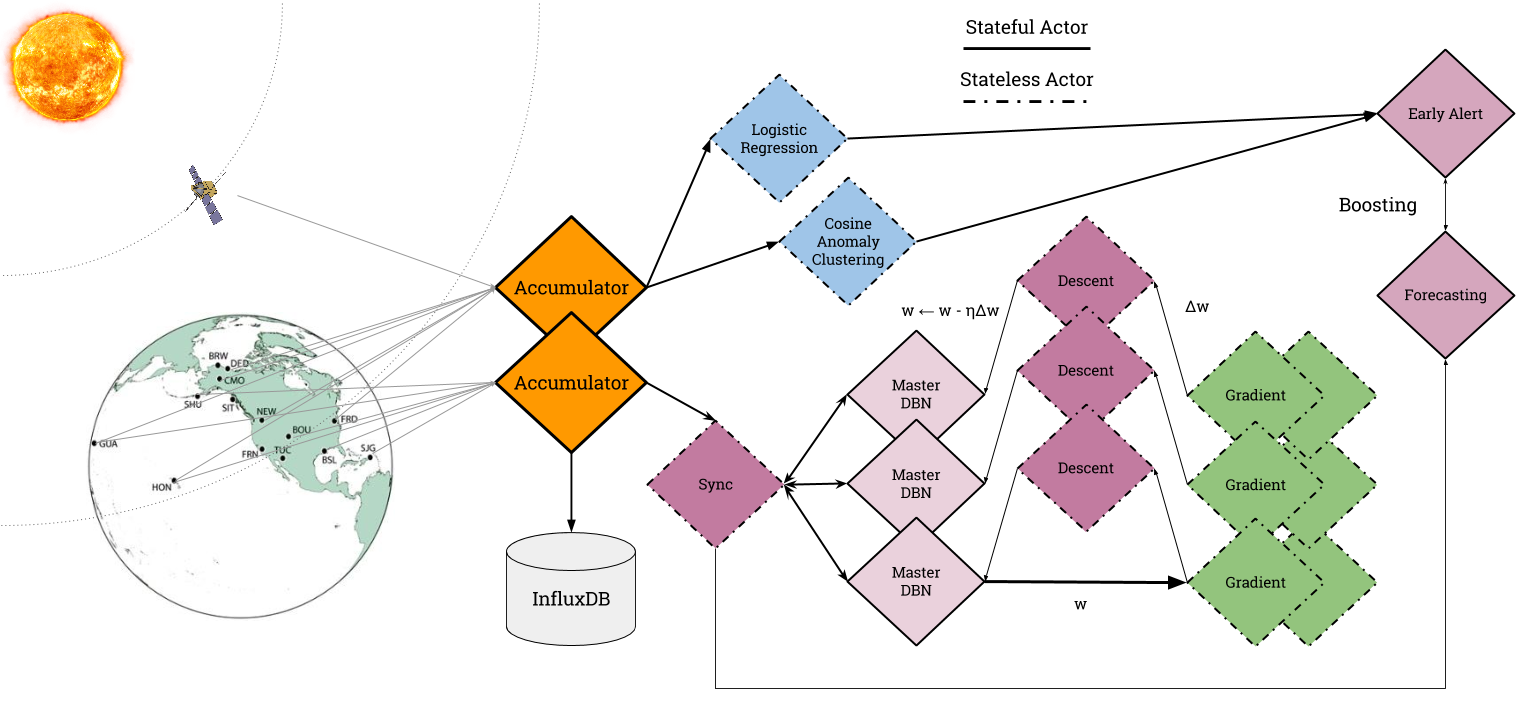
\includegraphics[width=0.45\textwidth]{solar_cast}
    \caption{The actor cast for a bagging approach to multiple machine learning models for solar flare prediction.}
    \label{fig:solar_cast}
\end{figure}

\subsection{Communication Pattern Analysis}

%TODO: This figures look weird. They need scaling to make them the right size.
\begin{figure*}[!t]
    \centering
    \subfloat[Email Dataflow]{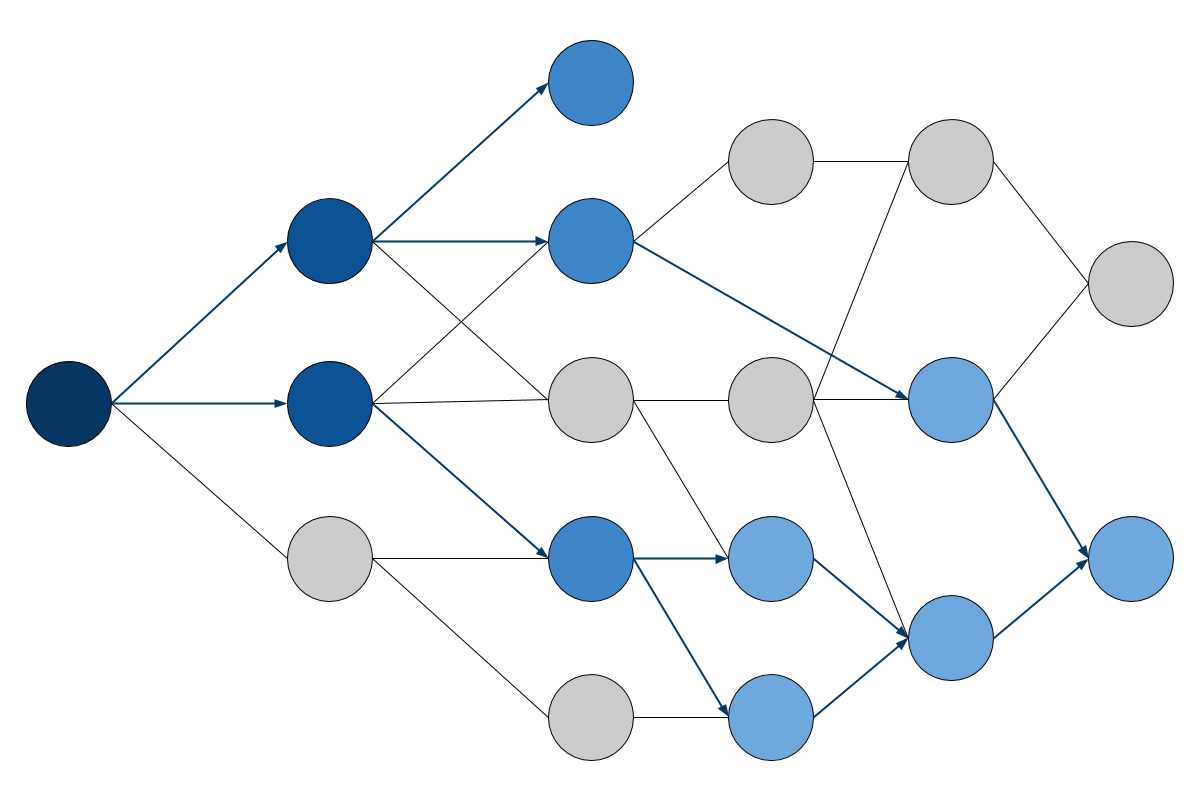
\includegraphics[width=0.3\textwidth]{dataflow_comms}
    \label{fig:dataflow_comms}}
    \hfil
    \subfloat[Online Recommendation]{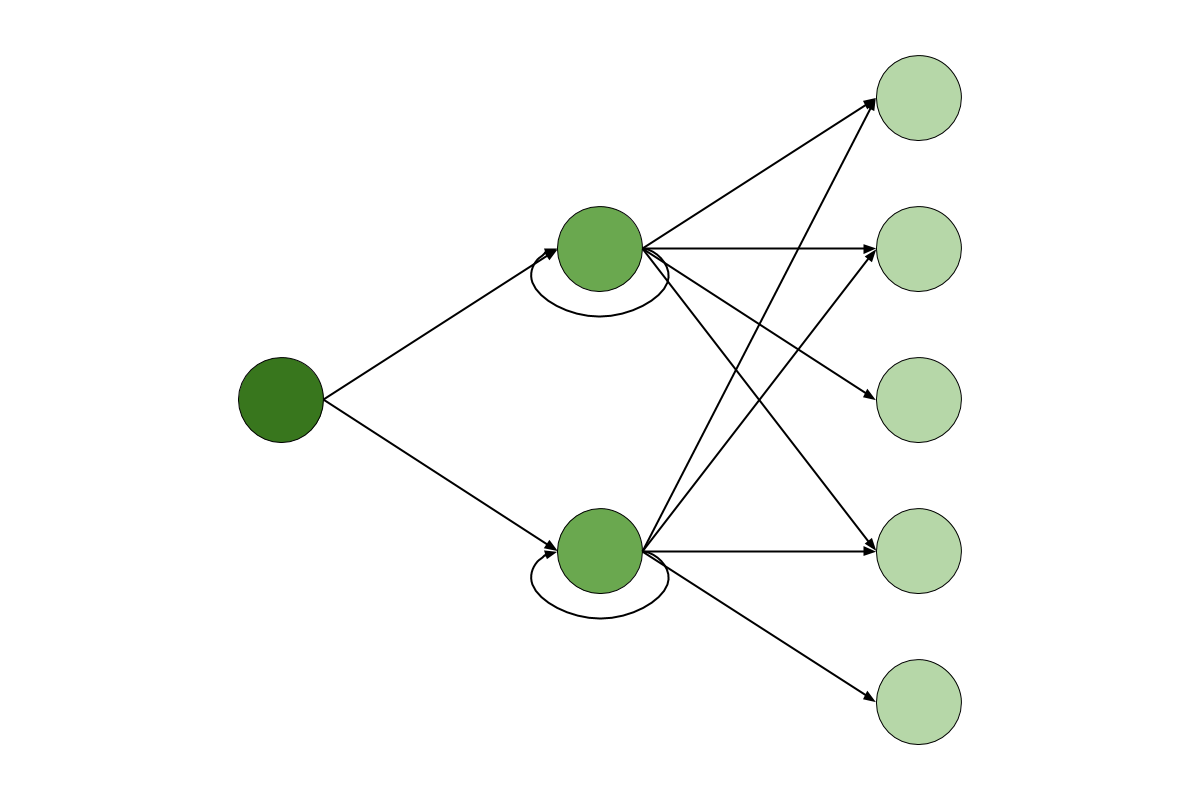
\includegraphics[width=0.3\textwidth]{nnmf_comms}
    \label{fig:nnmf_comms}}
    \hfil
    \subfloat[Solar Prediction]{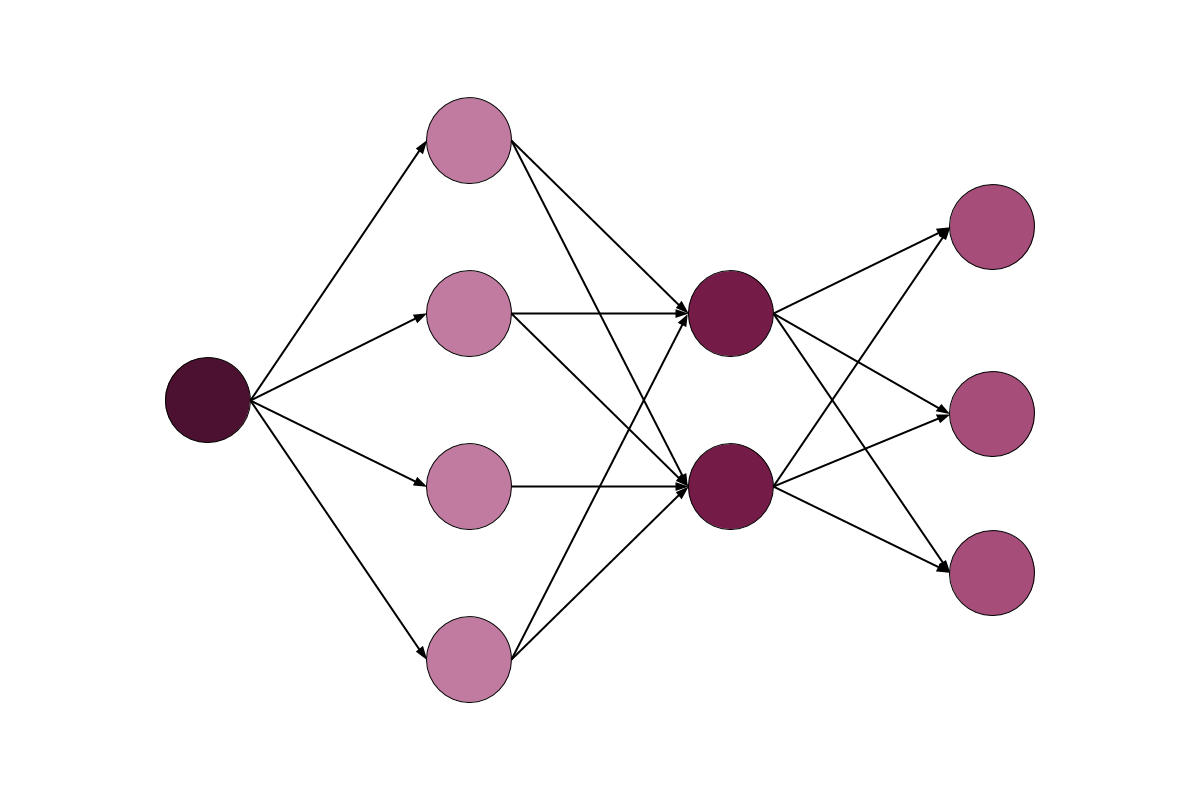
\includegraphics[width=0.3\textwidth]{solar_comms}
    \label{fig:solar_comms}}
    \caption{The corresponding communications patterns that we developed from these applications included branching, partial communication, iterative, front-loaded communication, and multiple-channel, full communication.}
    \label{fig:communications_patterns}
\end{figure*}

% TODO: this paragraph needs help
Through the analysis of these applications, which were selected to represent a variety of workflows and computational challenges, we noticed that the data flow of each represented different communication patterns. Because actors and distributed computing in general are inherently about communication, our approach became to first model the application as an actor cast, then once the cast had been finalized, to abstract the cast into a general communication pattern. We then used these general communication patterns to simulate traffic on a cluster of actors and show how a general actor space could be used for load balancing and scaling.

Described in detail in the following sections, the three applications are as follows: (1) a traditional data flow for real-time email analysis of a corporate network, (2) realtime recommendations an online store, and (3) solar flare prediction using deep belief networks and magnetometers. The corresponding communications patterns that we developed from these applications included branching, partial communication, iterative, front-loaded communication, and multiple-channel, full communication.

\section{Simulation Methodology}

Simpy \cite{matloff_introduction_2008}

\begin{figure}[!h]
    \centering
    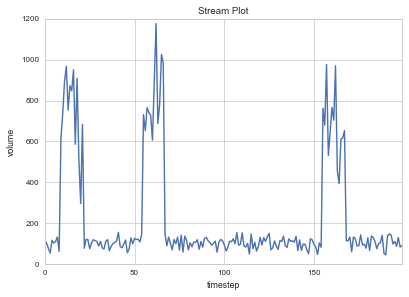
\includegraphics[width=0.45\textwidth]{streaming}
    \caption{Variable streaming data source with spikes of high activity, and longer periods of normal activity.}
    \label{fig:streaming}
\end{figure}

Our streaming data simulation is shown in Figure \ref{fig:streaming}.

% TODO: Cluster framework and representation
% TODO: Parameters for the simulation (streaming is already above)
% TODO: Discuss evaluation metric, utilization

\section{Discussion}

% TODO: Discuss what we learned
% TODO: Future work, etc.

If the number of available actors doesn't exceed the expected traffic, then the queue will continue to grow; forcing a reconfiguration.

\section{Conclusion}
The conclusion goes here.

% This should be very brief



% conference papers do not normally have an appendix


% use section* for acknowledgment
\section*{Acknowledgment}
We would like to thank Dr. Josh Rigler from USGS for discussing the magnetometer project with us, the available data sources and how it could be computed upon. We would also like to thank Dr. Michael Wiltberger from NCAR as well as Dr. Alan Susman from UMD who put us in touch with Dr. Rigler. Finally we'd like to thank Dr. Amol Deshpande for taking a look at our work and inspiring the initial actor model research.

% begin the references section.
\bibliographystyle{IEEEtran}
\bibliography{IEEEabrv,paper}



% that's all folks
\end{document}
